\section{\texorpdfstring{Přerušení}{Preruseni}}

% =====================================================================================================================
	\begin{frame}
    \frametitle{Přerušovací systém procesoru}
		
		\begin{itemize}
			\item zajišťuje reakci na asynchronní (často vnější) událost,
			\item při události je přerušeno vykonávání stávajícího programu a přejde se k „obsluze“ této události,
			\item po skončení přerušení se vrací procesor tam, kde opustil původní program,
			\item u každého MCU existuje způsob jak globálně všechny zdroje přerušení povolit i zakázat (globální povolení).
		\end{itemize}
		
		\begin{center}
			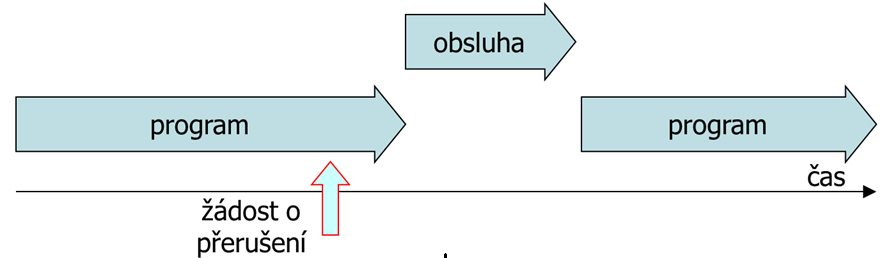
\includegraphics[width=0.90\textwidth]{fig/preruseni.png}
		\end{center}
		

	\end{frame}
	
% =====================================================================================================================
	\begin{frame}
    \frametitle{Vznik žádosti o přerušení}
		
		\small
		
		\begin{center}
			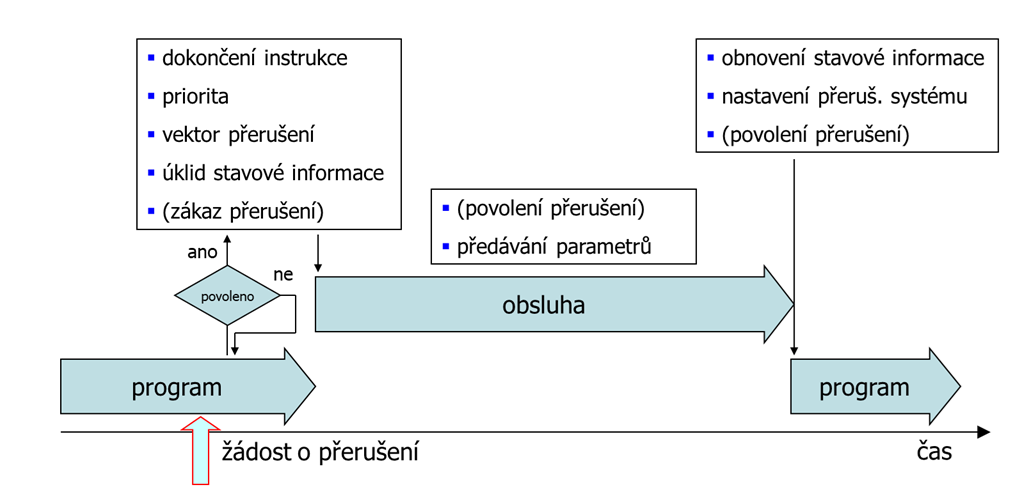
\includegraphics[width=1\textwidth]{fig/preruseni-podrobne.png}
		\end{center}
		
		\begin{itemize}
			\item U většiny zdrojů je nutné přerušení povolit - \textbf{maskovatelné přerušení},
			\item výjimkou je například SW přerušení TRAP - \textbf{nemaskovatelné přerušení}.
		\end{itemize}

	\end{frame}
	
% =====================================================================================================================
	\begin{frame}
    \frametitle{Zpracování více žádostí}
		
		\small
		
		\begin{center}
			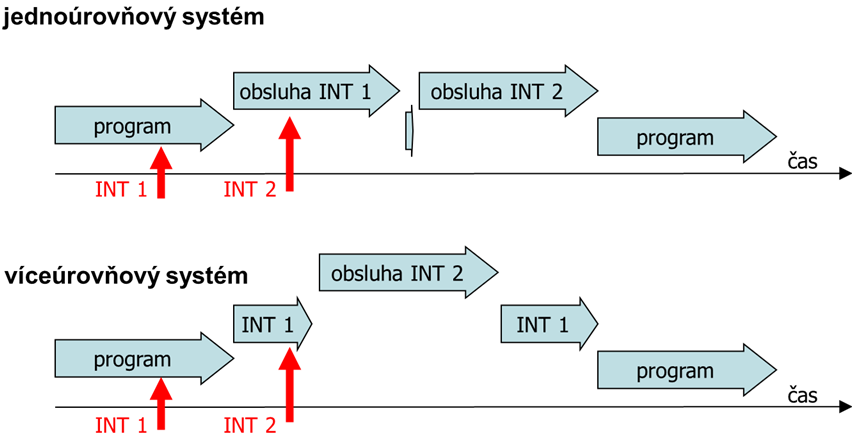
\includegraphics[width=0.9\textwidth]{fig/preruseni-systemy.png}
		\end{center}
		
		\begin{itemize}
			\item \textbf{MCU STM8} využívají víceúrovňový systém se \textbf{3 úrovněmi} a
			\item možností nastavení \textbf{priorit} jednotlivých žádostí.
		\end{itemize}

	\end{frame}
	
% =====================================================================================================================
	\begin{frame}
    \frametitle{STM8 - Vektor přerušení}
		\small
		\begin{itemize}
			\item je adresa (ukazatel) v paměti, na kterou procesor skočí při vzniku konkrétního přerušení, aby začal vykonávat obslužnou rutinu,
			\item naprosto základním \textbf{vektorem} je \textbf{RESET MCU} - určuje, odkud se začne vykonávat program viz obr.,
		\end{itemize}
		
		\begin{center}
			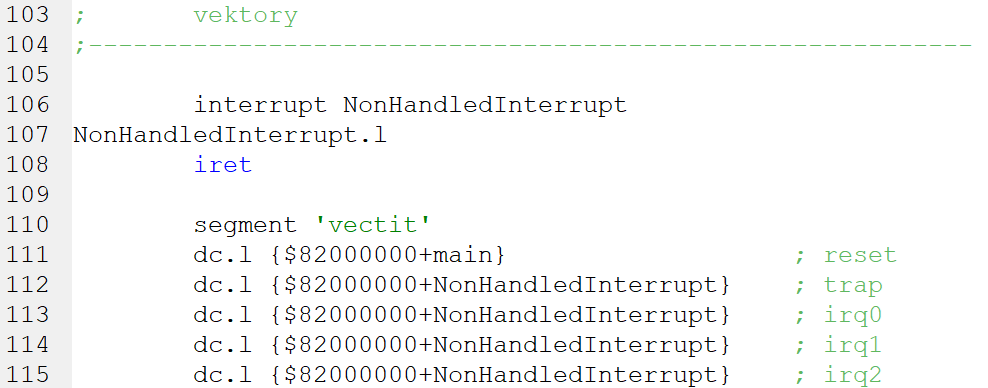
\includegraphics[width=0.9\textwidth]{fig/prg_vektory.png}
		\end{center}
		
		
		\begin{itemize}
			\item \textbf{0x82} je vyhrazený strojový kód vektoru následovaný 24 bit adresou \textbf{PCE:PCH:PCL}
		\end{itemize}

	\end{frame}
	
% =====================================================================================================================
	\begin{frame}
    \frametitle{STM8 - Zdroje přerušení}
		\small
		
		\begin{center}
			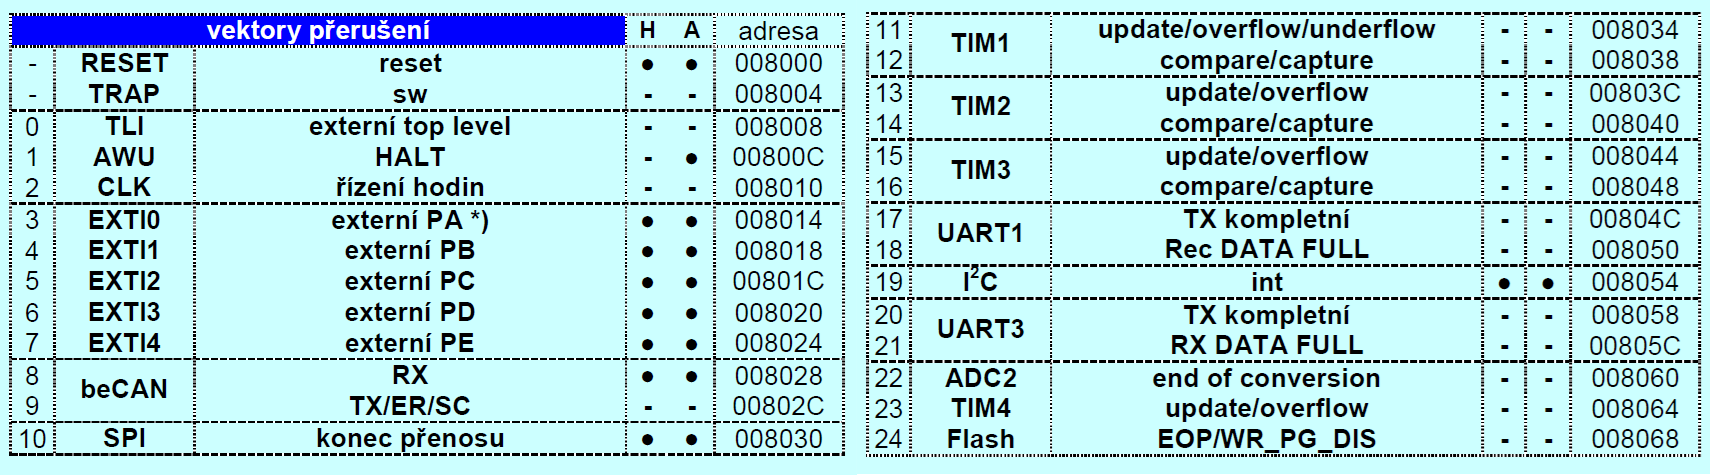
\includegraphics[width=\textwidth]{fig/preruseni-zdroje.png}
		\end{center}
		
		
		\begin{itemize}
			\item Adresa každého vektoru má přesně 4 byte (důvod viz předchozí slide),
			\item počátek vektorů je na adrese 0x8000,
			\item jeden vektor náleží jedné periférii, ale může reprezentovat více funkcí dané periférie (viz například \textbf{TIM1}, \textbf{TIM2},...)
		\end{itemize}

	\end{frame}
	
% =====================================================================================================================
	\begin{frame}
    \frametitle{STM8 - Povolení přerušení}
		\small
		
		\begin{enumerate}
			\item Předně je nutné povolit přerušení u dané periférie v příslušném registru (například u \textbf{ADC} je to \textbf{ADC\_CSR}),
			\item následně definovat prioritu, pokud využíváme víceúrovňový systém,
			\item nakonec globálně povolit vybavení přerušení (viz příznakový registr CC).
		\end{enumerate}
		
		\begin{center}
		\textbf{CC}
			\begin{tabular}{| p{5mm} | p{5mm} | p{5mm} | p{5mm} | p{5mm} | p{5mm} | p{5mm} | p{5mm} |}
				\hline
				\textbf{V} &  & \textcolor{red}{\textbf{I1}} & \textbf{H} & \textcolor{red}{\textbf{I0}} & \textbf{N} & \textbf{Z} & \textbf{C} \\
				\hline
			\end{tabular}
		\end{center}
		
		Úrovně na základě stavu bitů \textbf{I1}:\textbf{I0}
		\begin{center}
			\begin{tabular}{| c | c | l | c |}
				\hline
				\textbf{I1} & \textbf{I0} & \textbf{úroveň} & \textbf{instrukce} \\
				\hline
				$1$ & $0$ & hl. smyčka, přerušení povoleno & \textbf{RIM} \\
				$0$ & $1$ & úroveň 1 &  \\
				$0$ & $0$ & úroveň 2, vyšší priorita &  \\
				$1$ & $1$ & úroveň 3, přerušení zakázáno & \textbf{SIM} \\
				\hline
			\end{tabular}
		\end{center}
		
	\end{frame}
	
% =====================================================================================================================
	\begin{frame}
    \frametitle{STM8 - Nastavení priority přerušení}
		\small
		Registry \textbf{ITC\_SPRx}:
		\begin{center}
			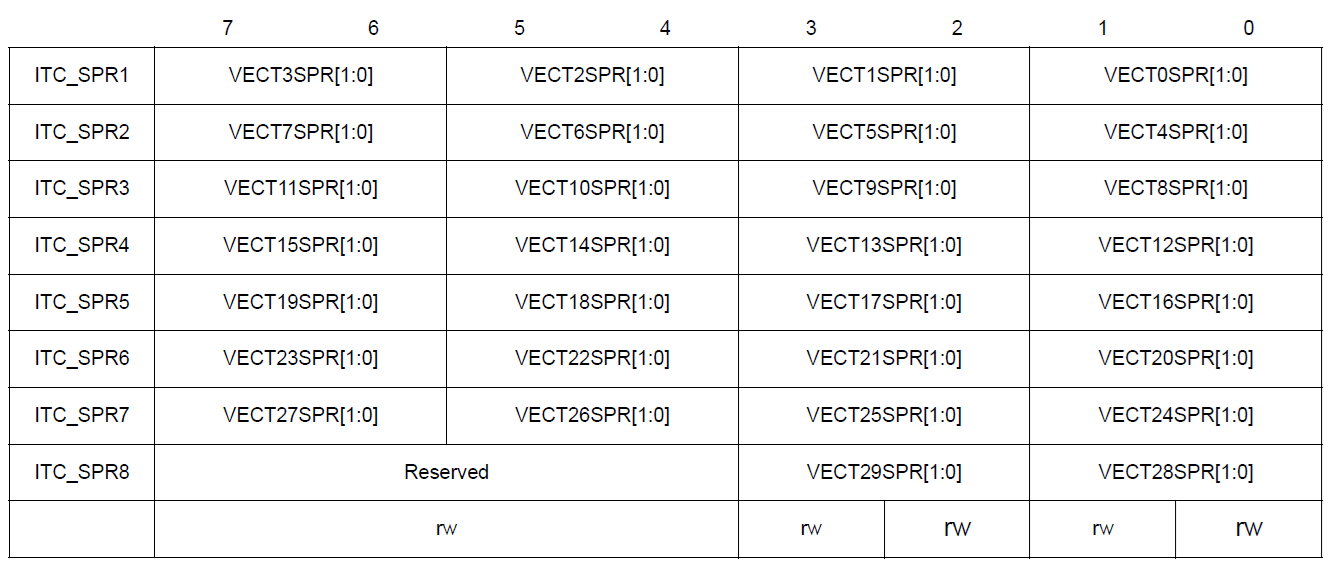
\includegraphics[width=\textwidth]{fig/ITC_SPRx.png}
		\end{center}
		
		\begin{itemize}
			\item Každému vektoru odpovídají 2 bity - kombinace \textbf{I1}:\textbf{I0},
			\item počáteční hodnota všech registrů po resetu je \textbf{0xFF}.
		\end{itemize}

	\end{frame}
	
% =====================================================================================================================
	\begin{frame}
    \frametitle{STM8 - Obsluha přerušení}
		\small
		\begin{center}
			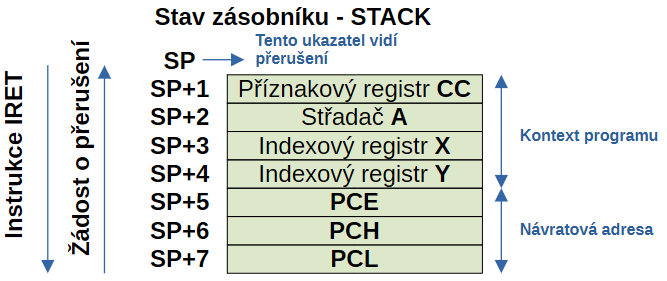
\includegraphics[width=0.9\textwidth]{fig/interrupt_stack.png}
		\end{center}
		
		\begin{itemize}
			\item Kromě návratové adresy se do zásobníku ukládá také kontext programu, aby přerušení neměnilo hodnotu \textbf{CPU registrů} pro hlavní program,
			\item návrat z přerušení zajišťuje instrukce \textcolor{blue}{\textbf{IRET}} 
		\end{itemize}

	\end{frame}